\documentclass{beamer}
\usepackage[utf8]{inputenc}

\usetheme{Madrid}
\usecolortheme{default}
\usepackage{amsmath,amssymb,amsfonts,amsthm}
\usepackage{txfonts}
\usepackage{tkz-euclide}
\usepackage{listings}
\usepackage{adjustbox}
\usepackage{array}
\usepackage{tabularx}
\usepackage{gvv}
\usepackage{lmodern}
\usepackage{circuitikz}
\usepackage{tikz}
\usepackage{graphicx}
\usepackage{multicol}

\setbeamertemplate{page number in head/foot}[totalframenumber]

\usepackage{tcolorbox}
\tcbuselibrary{minted,breakable,xparse,skins}



\definecolor{bg}{gray}{0.95}
\DeclareTCBListing{mintedbox}{O{}m!O{}}{%
  breakable=true,
  listing engine=minted,
  listing only,
  minted language=#2,
  minted style=default,
  minted options={%
    linenos,
    gobble=0,
    breaklines=true,
    breakafter=,,
    fontsize=\small,
    numbersep=8pt,
    #1},
  boxsep=0pt,
  left skip=0pt,
  right skip=0pt,
  left=25pt,
  right=0pt,
  top=3pt,
  bottom=3pt,
  arc=5pt,
  leftrule=0pt,
  rightrule=0pt,
  bottomrule=2pt,
  toprule=2pt,
  colback=bg,
  colframe=orange!70,
  enhanced,
  overlay={%
    \begin{tcbclipinterior}
    \fill[orange!20!white] (frame.south west) rectangle ([xshift=20pt]frame.north west);
    \end{tcbclipinterior}},
  #3,
}
\lstset{
    language=C,
    basicstyle=\ttfamily\small,
    keywordstyle=\color{blue},
    stringstyle=\color{orange},
    commentstyle=\color{green!60!black},
    numbers=left,
    numberstyle=\tiny\color{gray},
    breaklines=true,
    showstringspaces=false,
}
%------------------------------------------------------------
%This block of code defines the information to appear in the
%Title page
\title %optional
{4.13.34}
\date{September 30,2025}


\author 
{Jnanesh Sathisha karmar - EE25BTECH11029}



\begin{document}



\frame{\titlepage}
\begin{frame}{Question}The equations to a pair of opposite sides of parallogram are $x^2 - 5x + 6 = 0$ and $y^2 - 6y + 5 = 0$, the equations to its diagonals are
\begin{enumerate}
\begin{multicols}{2}
    \item $x+4y=13,y=4x-7$
    \item $4x+y=13,y=4x-7$
    \item $4x+y=13,4y=x-7$
    \item $y-4x=13,y+4x=7$
\end{multicols}
\end{enumerate}


\end{frame}



\begin{frame}{Equation}
 Given details\\Equation 1:
\begin{align}
   x^2-5x+6=0\\
   \text{This equation can be factored into:}\\
   \brak{x-2}\brak{x-3}=0\\
   \text{This gives us two vertical lines:}\\
   x=2\\
   x=3
\end{align}
\end{frame}
\begin{frame}{Equation}
Equation 2:
\begin{align}
    y^2-6y+5=0\\
    \text{This equation can be factored into:}\\
    \brak{y-1}\brak{y-5}=0\\
    \text{This gives us two horizontal lines:}\\
    y=1\\
    y=5
\end{align}
\end{frame}
\begin{frame}{Theoretical Solution}
Through the intersection of these 4 lines we can find the 4 vertices of the parallelogram 
\begin{align}
    \text{Intersection of}\  x=2\  \text{and}\  y=1 \text{is the point} \brak{2,1}.\text{Let vector}\ \vec{A}=\myvec{2\\1}\\
    \text{Intersection of}\  x=3\  \text{and}\  y=1 \text{is the point} \brak{3,1}.\text{Let vector}\ \vec{B}=\myvec{3\\1}\\
    \text{Intersection of}\  x=3\  \text{and}\  y=5 \text{is the point} \brak{3,5}.\text{Let vector}\ \vec{C}=\myvec{3\\5}\\
    \text{Intersection of}\  x=2\  \text{and}\  y=5 \text{is the point} \brak{2,5}.\text{Let vector}\ \vec{D}=\myvec{2\\5}\\
\end{align}
\end{frame}

\begin{frame}{Theoretical Solution}
The equations of the diagonals can be found using the matrix method. The equation of a line through $\brak{x_1, y_1}$ and $\brak{x_2, y_2}$ is given by setting the determinant of the matrix of coordinates to zero, as three collinear points form a triangle with zero area.
\begin{align*}
    \det \myvec{ x & y & 1 \\ x_1 & y_1 & 1 \\ x_2 & y_2 & 1 } = 0
\end{align*}
    
\end{frame}
\begin{frame}{Theoretical Solution}
The equation of the diagonal $\vec{AC}$, passing through $\vec{A}\brak{2, 1}$ and $\vec{C}$$\brak{3, 5}$, is:
\begin{align}
    \det \myvec{ x & y & 1 \\ 2 & 1 & 1 \\ 3 & 5 & 1 } &= 0 \\
    x\brak{1 \cdot 1 - 5 \cdot 1} - y\brak{2 \cdot 1 - 3 \cdot 1} + 1\brak{2 \cdot 5 - 3 \cdot 1} &= 0 \\
    x\brak{1 - 5} - y\brak{2 - 3} + 1\brak{10 - 3} &= 0 \\
    -4x - y\brak{-1} + 7 &= 0 \\
    -4x + y + 7 &= 0 \\
    y &= 4x - 7
\end{align}
\end{frame}
\begin{frame}{Theoretical Solution}
The equation of the diagonal $\vec{BD}$, passing through $\vec{B}$$\brak{3, 1}$ and $\vec{D}$$\brak{2, 5}$, is:
\begin{align}
    \det \myvec{ x & y & 1 \\ 3 & 1 & 1 \\ 2 & 5 & 1 } &= 0 \\
    x\brak{1 \cdot 1 - 5 \cdot 1} - y\brak{3 \cdot 1 - 2 \cdot 1} + 1\brak{3 \cdot 5 - 2 \cdot 1} &= 0 \\
    x\brak{1 - 5} - y\brak{3 - 2} + 1\brak{15 - 2} &= 0 \\
    -4x - y\brak{1} + 13 &= 0 \\
    -4x - y + 13 &= 0 \\
    4x + y &= 13
\end{align}
\end{frame}
\begin{frame}{Theoretical Solution}
Therefore the equations of both the diagonals are:
\begin{align}
    y=4x-7\\4x+y=13
\end{align}
Hence the answer is option 2
\end{frame}





\begin{frame}[fragile]
    \frametitle{C Code (1) - Function to store the points }

    \begin{lstlisting}
#include <stddef.h>

void find_diagonals(double x1, double x2, double y1, double y2, double* diag1_coeffs, double* diag2_coeffs) {
    if (diag1_coeffs == NULL || diag2_coeffs == NULL) {
        return;
    }

    diag1_coeffs[0] = y2 - y1;
    diag1_coeffs[1] = x1 - x2;
    diag1_coeffs[2] = (x2 * y1) - (x1 * y2);

    diag2_coeffs[0] = y1 - y2;
    diag2_coeffs[1] = x1 - x2;
    diag2_coeffs[2] = (x2 * y2) - (x1 * y1);
}


    \end{lstlisting}
\end{frame}

\begin{frame}[fragile]
    \frametitle{Python Code - Using Shared Object}
    \begin{lstlisting}
import ctypes
import numpy as np
import matplotlib.pyplot as plt
def solve_quadratic(a, b, c):
    discriminant = b**2 - 4*a*c
    if discriminant < 0:
        return None, None
    r1 = (-b + np.sqrt(discriminant)) / (2*a)
    r2 = (-b - np.sqrt(discriminant)) / (2*a)
    return r1, r2
def main():
    lib_path = "./diagonals.so"
    try:
        diag_lib = ctypes.CDLL(lib_path)
    except OSError as e:
        print(f"Error loading shared library: {e}")
        print("Please ensure 'diag_calculator.so' exists. You may need to compile the C code first using 'sh compile.sh'")
        return
\end{lstlisting}
\end{frame}

\begin{frame}[fragile]
    \frametitle{Python Code - Using Shared Object}
    \begin{lstlisting}
   diag_lib.find_diagonals.argtypes = [
        ctypes.c_double, ctypes.c_double,
        ctypes.c_double, ctypes.c_double,
        ctypes.POINTER(ctypes.c_double),
        ctypes.POINTER(ctypes.c_double)
    ]
    diag_lib.find_diagonals.restype = None

    x1, x2 = solve_quadratic(1, -5, 6)
    y1, y2 = solve_quadratic(1, -6, 5)

    if x1 is None or y1 is None:
        print("Error: Could not solve quadratic equations. Check coefficients.")
        return
\end{lstlisting}
\end{frame}
\begin{frame}[fragile]
    \frametitle{Python Code - Using Shared Object}
    \begin{lstlisting}
       print(f"Parallelogram lines: x={x1}, x={x2}, y={y1}, y={y2}")

    Diag1Coeffs = (ctypes.c_double * 3)()
    Diag2Coeffs = (ctypes.c_double * 3)()

    diag_lib.find_diagonals(x1, x2, y1, y2, Diag1Coeffs, Diag2Coeffs)

    d1 = [c for c in Diag1Coeffs]
    d2 = [c for c in Diag2Coeffs]
    print(f"Diagonal 1 (Ax+By+C=0): A={d1[0]:.1f}, B={d1[1]:.1f}, C={d1[2]:.1f}")
    print(f"Diagonal 2 (Ax+By+C=0): A={d2[0]:.1f}, B={d2[1]:.1f}, C={d2[2]:.1f}")
\end{lstlisting}
\end{frame}
\begin{frame}[fragile]
    \frametitle{Python Code - Using Shared Object}
    \begin{lstlisting}
fig, ax = plt.subplots(figsize=(8, 8))

    parallelogram_x = [x1, x2, x2, x1, x1]
    parallelogram_y = [y1, y1, y2, y2, y1]
    ax.plot(parallelogram_x, parallelogram_y, 'b-', label='Parallelogram Sides', linewidth=2)

    plot_x_range = np.linspace(min(x1, x2) - 1, max(x1, x2) + 1, 100)
    
    def plot_line(coeffs, style, label):
        A, B, C = coeffs
        if abs(B) > 0:
            y_vals = (-A * plot_x_range - C) / B
            ax.plot(plot_x_range, y_vals, style, label=label)
        else:
            x_val = -C / A
            ax.axvline(x=x_val, linestyle=style.strip('-'), color=style[0], label=label)
\end{lstlisting}
\end{frame}
\begin{frame}[fragile]
    \frametitle{Python Code - Using Shared Object}
    \begin{lstlisting}
    plot_line(d1, 'r--', 'Diagonal 1')
    plot_line(d2, 'g--', 'Diagonal 2')

    ax.set_title('Parallelogram and its Diagonals')
    ax.set_xlabel('X-axis')
    ax.set_ylabel('Y-axis')
    ax.grid(True, linestyle=':', alpha=0.6)
    ax.legend()
    
    padding = 2
    ax.set_xlim(min(x1, x2) - padding, max(x1, x2) + padding)
    ax.set_ylim(min(y1, y2) - padding, max(y1, y2) + padding)
    ax.set_aspect('equal', adjustable='box')
\end{lstlisting}
\end{frame}
\begin{frame}[fragile]
    \frametitle{Python Code - Using Shared Object}
    \begin{lstlisting}
    x_min, x_max = min(x1, x2), max(x1, x2)
    y_min, y_max = min(y1, y2), max(y1, y2)
    vertices = {'A':(x_min, y_min), 'B':(x_max, y_min), 'C':(x_max, y_max), 'D':(x_min, y_max)}
    for name, (px, py) in vertices.items():
        ax.plot(px, py, 'ko')
        ax.text(px + 0.1, py + 0.1, f'{name}({px:.1f},{py:.1f})')

    plt.savefig("./figs/diagonals.png") 
    subprocess.run(shlex.split('termux-open ../figs/diagonals.png'))
    plt.show()

if __name__ == "__main__":
    main()
\end{lstlisting}
\end{frame}

\begin{frame}{Plot-Using Both C and Python}
    \centering
    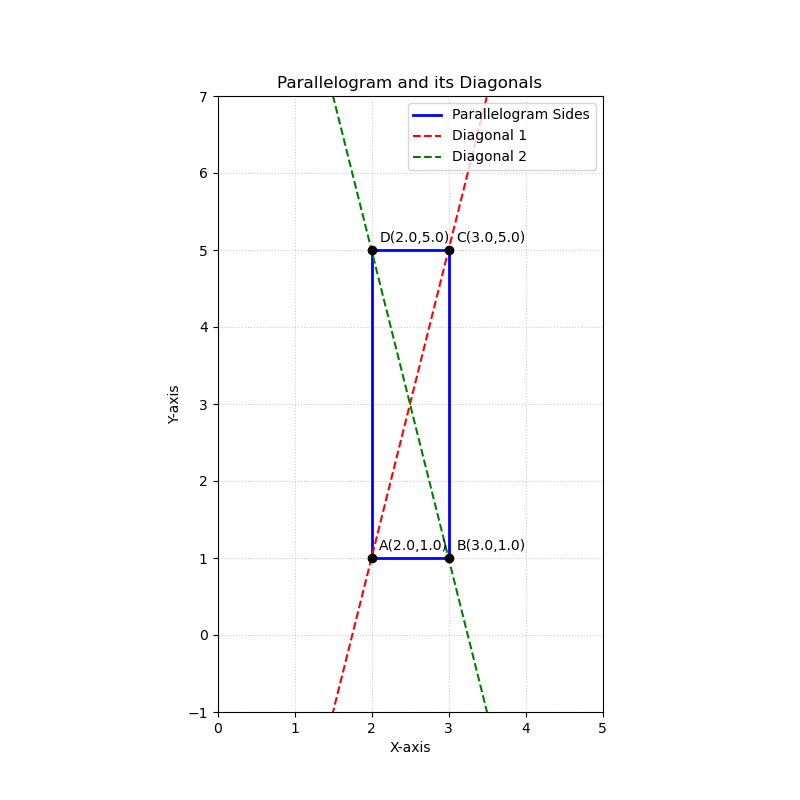
\includegraphics[width=\columnwidth, height=0.8\textheight, keepaspectratio]{figs/diagonals.png}     
\end{frame}

\begin{frame}[fragile]
    \frametitle{Python Code}
    \begin{lstlisting}
import numpy as np
import matplotlib.pyplot as plt

def solve_quadratic(a, b, c):
    discriminant = b**2 - 4*a*c
    if discriminant < 0:
        return None, None
    r1 = (-b + np.sqrt(discriminant)) / (2*a)
    r2 = (-b - np.sqrt(discriminant)) / (2*a)
    return r1, r2

def find_diagonals_python(x1, x2, y1, y2):
    A1 = y2 - y1
    B1 = x1 - x2
    C1 = (x2 * y1) - (x1 * y2)
    diag1_coeffs = [A1, B1, C1]
\end{lstlisting}
\end{frame}
\begin{frame}[fragile]
    \frametitle{Python Code}
    \begin{lstlisting}
    A2 = y1 - y2
    B2 = x1 - x2
    C2 = (x2 * y2) - (x1 * y1)
    diag2_coeffs = [A2, B2, C2]
    
    return diag1_coeffs, diag2_coeffs

def main():
    x1, x2 = solve_quadratic(1, -5, 6)
    y1, y2 = solve_quadratic(1, -6, 5)

    if x1 is None or y1 is None:
        print("Error: Could not solve quadratic equations. Check coefficients.")
        return
\end{lstlisting}
\end{frame}
\begin{frame}[fragile]
    \frametitle{Python Code}
    \begin{lstlisting}
    print(f"Parallelogram lines: x={x1}, x={x2}, y={y1}, y={y2}")

    d1, d2 = find_diagonals_python(x1, x2, y1, y2)
    
    print(f"Diagonal 1 (Ax+By+C=0): A={d1[0]:.1f}, B={d1[1]:.1f}, C={d1[2]:.1f}")
    print(f"Diagonal 2 (Ax+By+C=0): A={d2[0]:.1f}, B={d2[1]:.1f}, C={d2[2]:.1f}")

    fig, ax = plt.subplots(figsize=(8, 8))

    parallelogram_x = [x1, x2, x2, x1, x1]
    parallelogram_y = [y1, y1, y2, y2, y1]
    ax.plot(parallelogram_x, parallelogram_y, 'b-', label='Parallelogram Sides', linewidth=2)
\end{lstlisting}
\end{frame}
\begin{frame}[fragile]
    \frametitle{Python Code}
    \begin{lstlisting}
    plot_x_range = np.linspace(min(x1, x2) - 1, max(x1, x2) + 1, 100)
    
    def plot_line(coeffs, style, label):
        A, B, C = coeffs
        if abs(B) > 0:
            y_vals = (-A * plot_x_range - C) / B
            ax.plot(plot_x_range, y_vals, style, label=label)
        else:
            x_val = -C / A
            ax.axvline(x=x_val, linestyle=style.strip('-'), color=style[0], label=label)

    plot_line(d1, 'r--', 'Diagonal 1')
    plot_line(d2, 'g--', 'Diagonal 2')
\end{lstlisting}
\end{frame}
\begin{frame}[fragile]
    \frametitle{Python Code}
    \begin{lstlisting}
    ax.set_title('Parallelogram and its Diagonals')
    ax.set_xlabel('X-axis')
    ax.set_ylabel('Y-axis')
    ax.grid(True, linestyle=':', alpha=0.6)
    ax.legend()
    
    padding = 2
    ax.set_xlim(min(x1, x2) - padding, max(x1, x2) + padding)
    ax.set_ylim(min(y1, y2) - padding, max(y1, y2) + padding)
    ax.set_aspect('equal', adjustable='box')
\end{lstlisting}
\end{frame}
\begin{frame}[fragile]
    \frametitle{Python Code}
    \begin{lstlisting}
    x_min, x_max = min(x1, x2), max(x1, x2)
    y_min, y_max = min(y1, y2), max(y1, y2)
    vertices = {'A':(x_min, y_min), 'B':(x_max, y_min), 'C':(x_max, y_max), 'D':(x_min, y_max)}
    for name, (px, py) in vertices.items():
        ax.plot(px, py, 'ko')
        ax.text(px + 0.1, py + 0.1, f'{name}({px:.1f},{py:.1f})')
    plt.savefig("./figs/diagonals2.png") 
    plt.show()

if __name__ == "__main__":
    main()

\end{lstlisting}
\end{frame}


\begin{frame}{Plot-Using only Python}
    \centering
    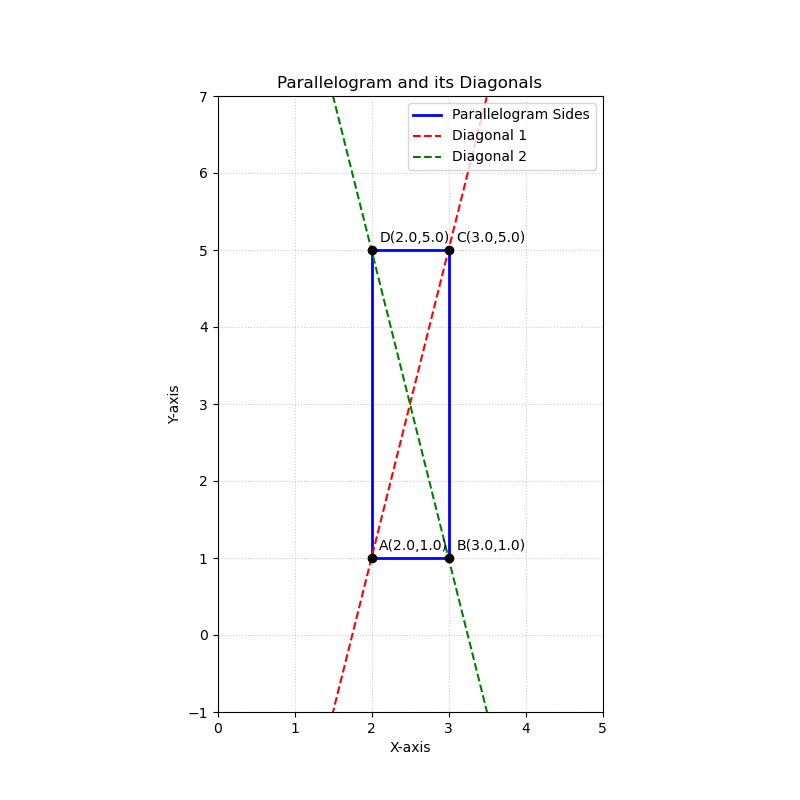
\includegraphics[width=\columnwidth, height=0.8\textheight, keepaspectratio]{figs/diagonals2.png}     
\end{frame}


\end{document}